\documentclass{mcmthesis}
\mcmsetup{CTeX = true,   % 使用 CTeX 套装时,设置为 true
        tcn = XJ162, problem = A,
        sheet = true, titleinsheet = true, keywordsinsheet = true,
        titlepage = false, abstract = false}
\geometry{left=1in,right=0.75in,top=1in,bottom=1in}
\numberwithin{figure}{section}
\numberwithin{table}{section}
\numberwithin{equation}{section}
\usepackage{newtxtext}
\usepackage{lipsum}
\usepackage{palatino}
\usepackage{hyperref}
\usepackage{booktabs}
\usepackage{subfigure}
\usepackage{graphicx}
\usepackage{pythonhighlight}
\usepackage{indentfirst}%首段自动缩进
\usepackage{colortbl}
\usepackage{apacite}
\usepackage{natbib}


\setlength{\parindent}{2em}
\title{test}
\setlength{\headheight}{15pt}

\definecolor{darkOrange}{rgb}{0.929,0.49,0.192}
\definecolor{Orange}{rgb}{0.973,0.796,0.678}
\definecolor{lightOrange}{rgb}{0.988,0.894,0.839}

\begin{document}

\begin{abstract}



\begin{keywords}
123456
\end{keywords}
\end{abstract}
\maketitle

\tableofcontents
  \thispagestyle{empty}
  \newpage
  \setcounter{page}{1}
%%
%%Generate the Memorandum, if it's needed.
%\memoto{\LaTeX{}studio}
%\memofrom{Liam Huang}
%\memosubject{Happy \TeX{}ing!}
%\memodate{\today}
%%\logo{\LARGE I'm pretending to be a LOGO!}
%\begin{memo}[Memorandum]
%  \lipsum[1-3]
%\end{memo}

\section{Introduction}

\subsection{Problem Restatement}

Finless porpoise is the only freshwater mammal in the Yangtze River at present, 
which is distributed in the middle and lower reaches of the Yangtze 
River, Dongting Lake and Poyang Lake, and its population has 
decreased dramatically in the past 20 years. According to the statistics, 
the number of finless porpoises in the Yangtze River was more than 2,700 in 1991. 
However, in the year of 2006, there were fewer than 1,800 finless porpoises surviving in the area. 
In 2011, there were probably just over 1,000 of them, and in 2018 there were about 1,012. 
\par
In fact, since the 1980s, the ecologists along with the government
had explored and developed three conservation strategies: 
in situ conservation, ex situ conservation and artificial breeding.
Among them, ex situ protection, that is, selecting some waters with 
similar ecological environment to the Yangtze River to establish 
ex situ protection, is the most direct and effective measure
to protect the Yangtze finless porpoise. 
\par
China has set up five ex-situ protected sites until now, in which 
more than 150 Yangtze finless porpoises are conserved. On September 18, 2021, CCTV reported that 
the population of the Yangtze finless porpoise is growing steadily. 
The population decline of the Yangtze finless porpoise has been 
curbed, but its critically endangered status remains unchanged.
\par
Based on what has been discussed above, please address the following problems:
\begin{enumerate}
  \item [1] Establish a mathematical model to predict the population number of finless porpoises in five ex situ protected areas after 20 years, 
  and explain how the sex ratio of 150 finless porpoises in ex situ protected areas affects the population development of finless porpoises.
  \item [2] Will the Yangtze finless porpoise become functionally extinct without ex situ conservation strategies?
  \item [3] Based on your analysis, please submit no more than 2 pages of recommendations for the protection of finless porpoises to the relevant authorities.
\end{enumerate}

\subsection{Overview of Our Work}




\section{Assumptions and Justifications}
These are necessary assumptions for simplifying the model.
\begin{enumerate}
  \item [1.] The carrying capacity per unit area of each ex-situ conservation layout is constant.
  \item [2.] 
\end{enumerate}


\section{Notations}

\renewcommand\arraystretch{1.5}

\begin{table}[htpb!]
  \centering
  \caption{Notation Descriptions} \label{Notation}
  \begin{tabular}{m{2.5cm}<{\centering}|m{12.5cm}<{\centering}}
  \toprule[1.5pt]
  \textbf{Symbol} & \textbf{Definition} \\ \hline
  $ r $ & Innate rate of increase \\
  %内廪增长率:给定的物理和生物的条件下,具有稳定的年龄组配的种群的最大瞬时增长率
  $ \lambda $ & Finite rate of increase \\
  %周限增长率:种群 不受资源限制的情况下,种群内平均每一个个体能产生的后代数
  $ R_\theta $ &  Intrinsic rate of natural increase\\
  %一定时间内种群中雌性个体能够产下的新生雌性个体总数的能力
   N-extant  & Average extant population size\\ 
   N-all  & Average population size \\
   PE  & Probability of Extinction \\
   GeneDiv  &  Genetic Diversity \\
   TE & Time of Extinction(year) \\
   SD & Standard Deviation \\
   $ K $ & Carrying capacity \\ 
   $ N_t $ & Size of finless porpoise population in the year of $ 1991 + t $ \\ 
  \bottomrule[1.5pt]
  \end{tabular}
  \end{table}



\section{Intorduction and Results of Models}

Note that because of the deficiency of the statistics about the other four ex-situ conservations,
the size of finless porpoise population per unit area is considered 
the same as that in Swan Oxbow of the Yangtse River.
\par
Considering tremendous cost on massive finless porpoise population 
census, merely six years of data was collected in Swan Oxbow of the Yangtse River
during the three decades since 1992. \citep{Liuzhigang}
Thus, we've applied \textbf{Lagrange interpolation} to obtain other years' data
in Swan Oxbow.



\subsection{Relation between Population size and Time based on Lagrange Interpolation}
Given $ n $ distinct real values $ x_1, x_2, \cdots , x_n $and $ n $
real values $ y_1, y_2,\cdots, y_n $ (not necessarily distinct), there
is a unique polynomial $ P $ with real coefficients satisfying 
$ P(x_i)= y_i $ for $ i \in \{1,2,\cdots,n\} $, such that deg($ P $ )<n.
\par
The polynomial $ P(x) $ is defined as follows:   
$$
  P(x) = \sum \limits _{k = 1}^ny_kp_k(x),\quad
  p_k(x) = \frac{(x-x_1)\cdots (x-x_{k-1})(x-x_{k+1})\cdots (x-x_n)}{
    (x_k-x_1)\cdots (x_k-x_{k-1})(x_k-x_{k+1})\cdots (x_k-x_n)
  }
$$

After substituted the number in 1992, 2002, 2005, 2007, 2015 and 2021,
the figure of the polynomial is as follows:
\begin{figure}[htbp!]
  \centering
  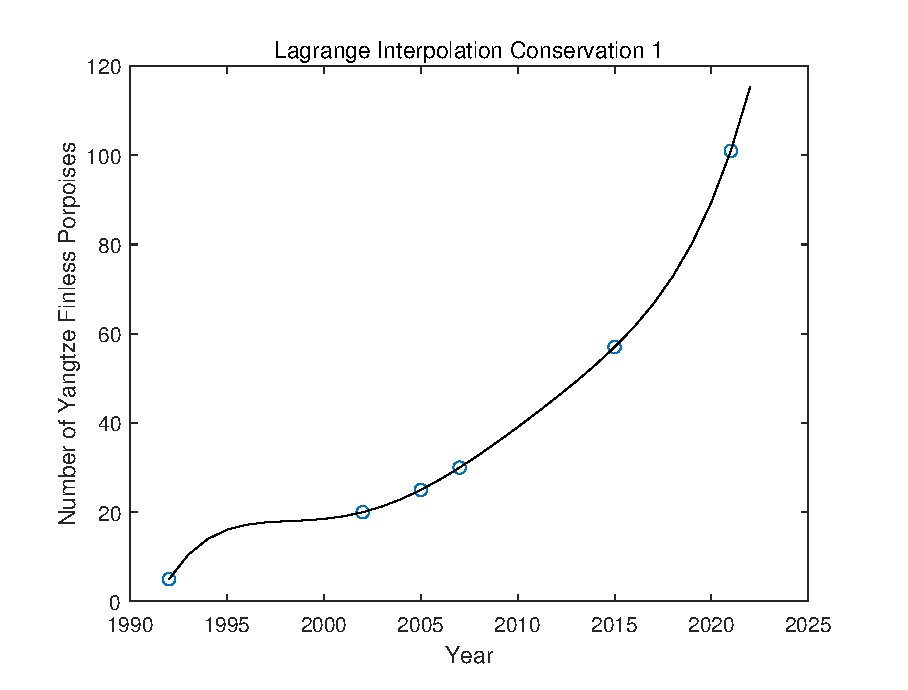
\includegraphics[width = 8cm]{codes/Lagrange.eps}
  \caption{Langrange Interpolation Conservation}
\end{figure}

\par
According to Lagrange interpolation and the definition of $ N_t $ :
$$
  N_t = P(t) \quad t = 1,\cdots ,30
$$ 
and the exact numbers are listed below:
\begin{table}[htpb!]
  \centering
  \caption{Estimated size of population on year basis from 1992 to 2022} \label{Lagrange table}
  \begin{tabular}{m{2cm}<{\centering}|m{2cm}<{\centering}|m{2cm}<{\centering}|m{2cm}<{\centering}|m{2cm}<{\centering}|m{2cm}<{\centering}}
  \rowcolor{darkOrange}  \textbf{Year}&\textbf{Number}&\textbf{Year}&\textbf{Number}&\textbf{Year}&\textbf{Number}\\ \hline
  \rowcolor{Orange}  1992 & 5       & 2002 & 20      & 2012 & 45.7364 \\
  \rowcolor{lightOrange}  1993 & 10.4864 & 2003 & 21.2919 & 2013 & 49.2555 \\
  \rowcolor{Orange}  1994 & 13.9987 & 2004 & 22.9647 & 2014 & 52.9737 \\
  \rowcolor{lightOrange}  1995 & 16.0839 & 2005 & 25      & 2015 & 57      \\
  \rowcolor{Orange}  1996 & 17.2014 & 2006 & 27.3612 & 2016 & 61.4941 \\
  \rowcolor{lightOrange}  1997 & 17.7296 & 2007 & 30      & 2017 & 66.6734 \\
  \rowcolor{Orange}  1998 & 17.9732 & 2008 & 32.8636 & 2018 & 72.82   \\
  \rowcolor{lightOrange}  1999 & 18.1701 & 2009 & 35.9015 & 2019 & 80.2876 \\
  \rowcolor{Orange}  2000 & 18.4981 & 2010 & 39.0724 & 2020 & 89.5084 \\
  \rowcolor{lightOrange}  2001 & 19.0819 & 2011 & 42.3514 & 2021 & 101     \\
  \end{tabular}
\end{table}

\subsection{Model I: Vortex model based finless porpoise analysis}








\subsection{Model II: Auto Regressive Integrated Moving Average(ARIMA) model}
We apply ARIMA model in order to predict the size of finless porpoise population in five ex-situ 
conservation areas after 20 years.
\par
\begin{minipage}[htbp]{0.35\linewidth}
  Under regular circumstances, the time series we obtain in the real world
  has tendency, seasonality and non-stationarity. Thus, it's vital for 
  us to transfer the non-stationary time series to stationary time series and 
  make an assumption that the time series is an Auto Regressive Moving Average
  (ARMA) series to predict the future data.  ARMA series is defined as follows.
  \begin{align*}
    &X_t-\phi_1X_{t-1}-\cdots -\phi_pX_{t-p} \\
    &= \epsilon_t - \theta_1\epsilon_{t-1}-\cdots-\theta_q\epsilon_{t-q}
  \end{align*}

$ \epsilon_1 $ is a stationary white noise whose average is zero and
deviation is $ \sigma_\epsilon^2 $;$ X_t $is an ARMA series with $ p $ and $ q $
degree, recorded briefly as $ \mathbf{ARMA}(p,q) $ series.
Akaike Information Criterion(AIC) is one of the most commonly used
criterion to determine the degree of $ \mathbf{ARMA}(p,q) $: choose 
$ p,q $ such that 
\begin{equation}\label{AIC}
  \begin{aligned}
    \min \mathbf{AIC} &= n\ln \hat{\sigma_\epsilon^2} \\
    &+ 2(p+q+1)
  \end{aligned}
\end{equation}

\end{minipage}
\hfill
\begin{minipage}[htbp]{0.55\linewidth}
  \begin{flushright}
    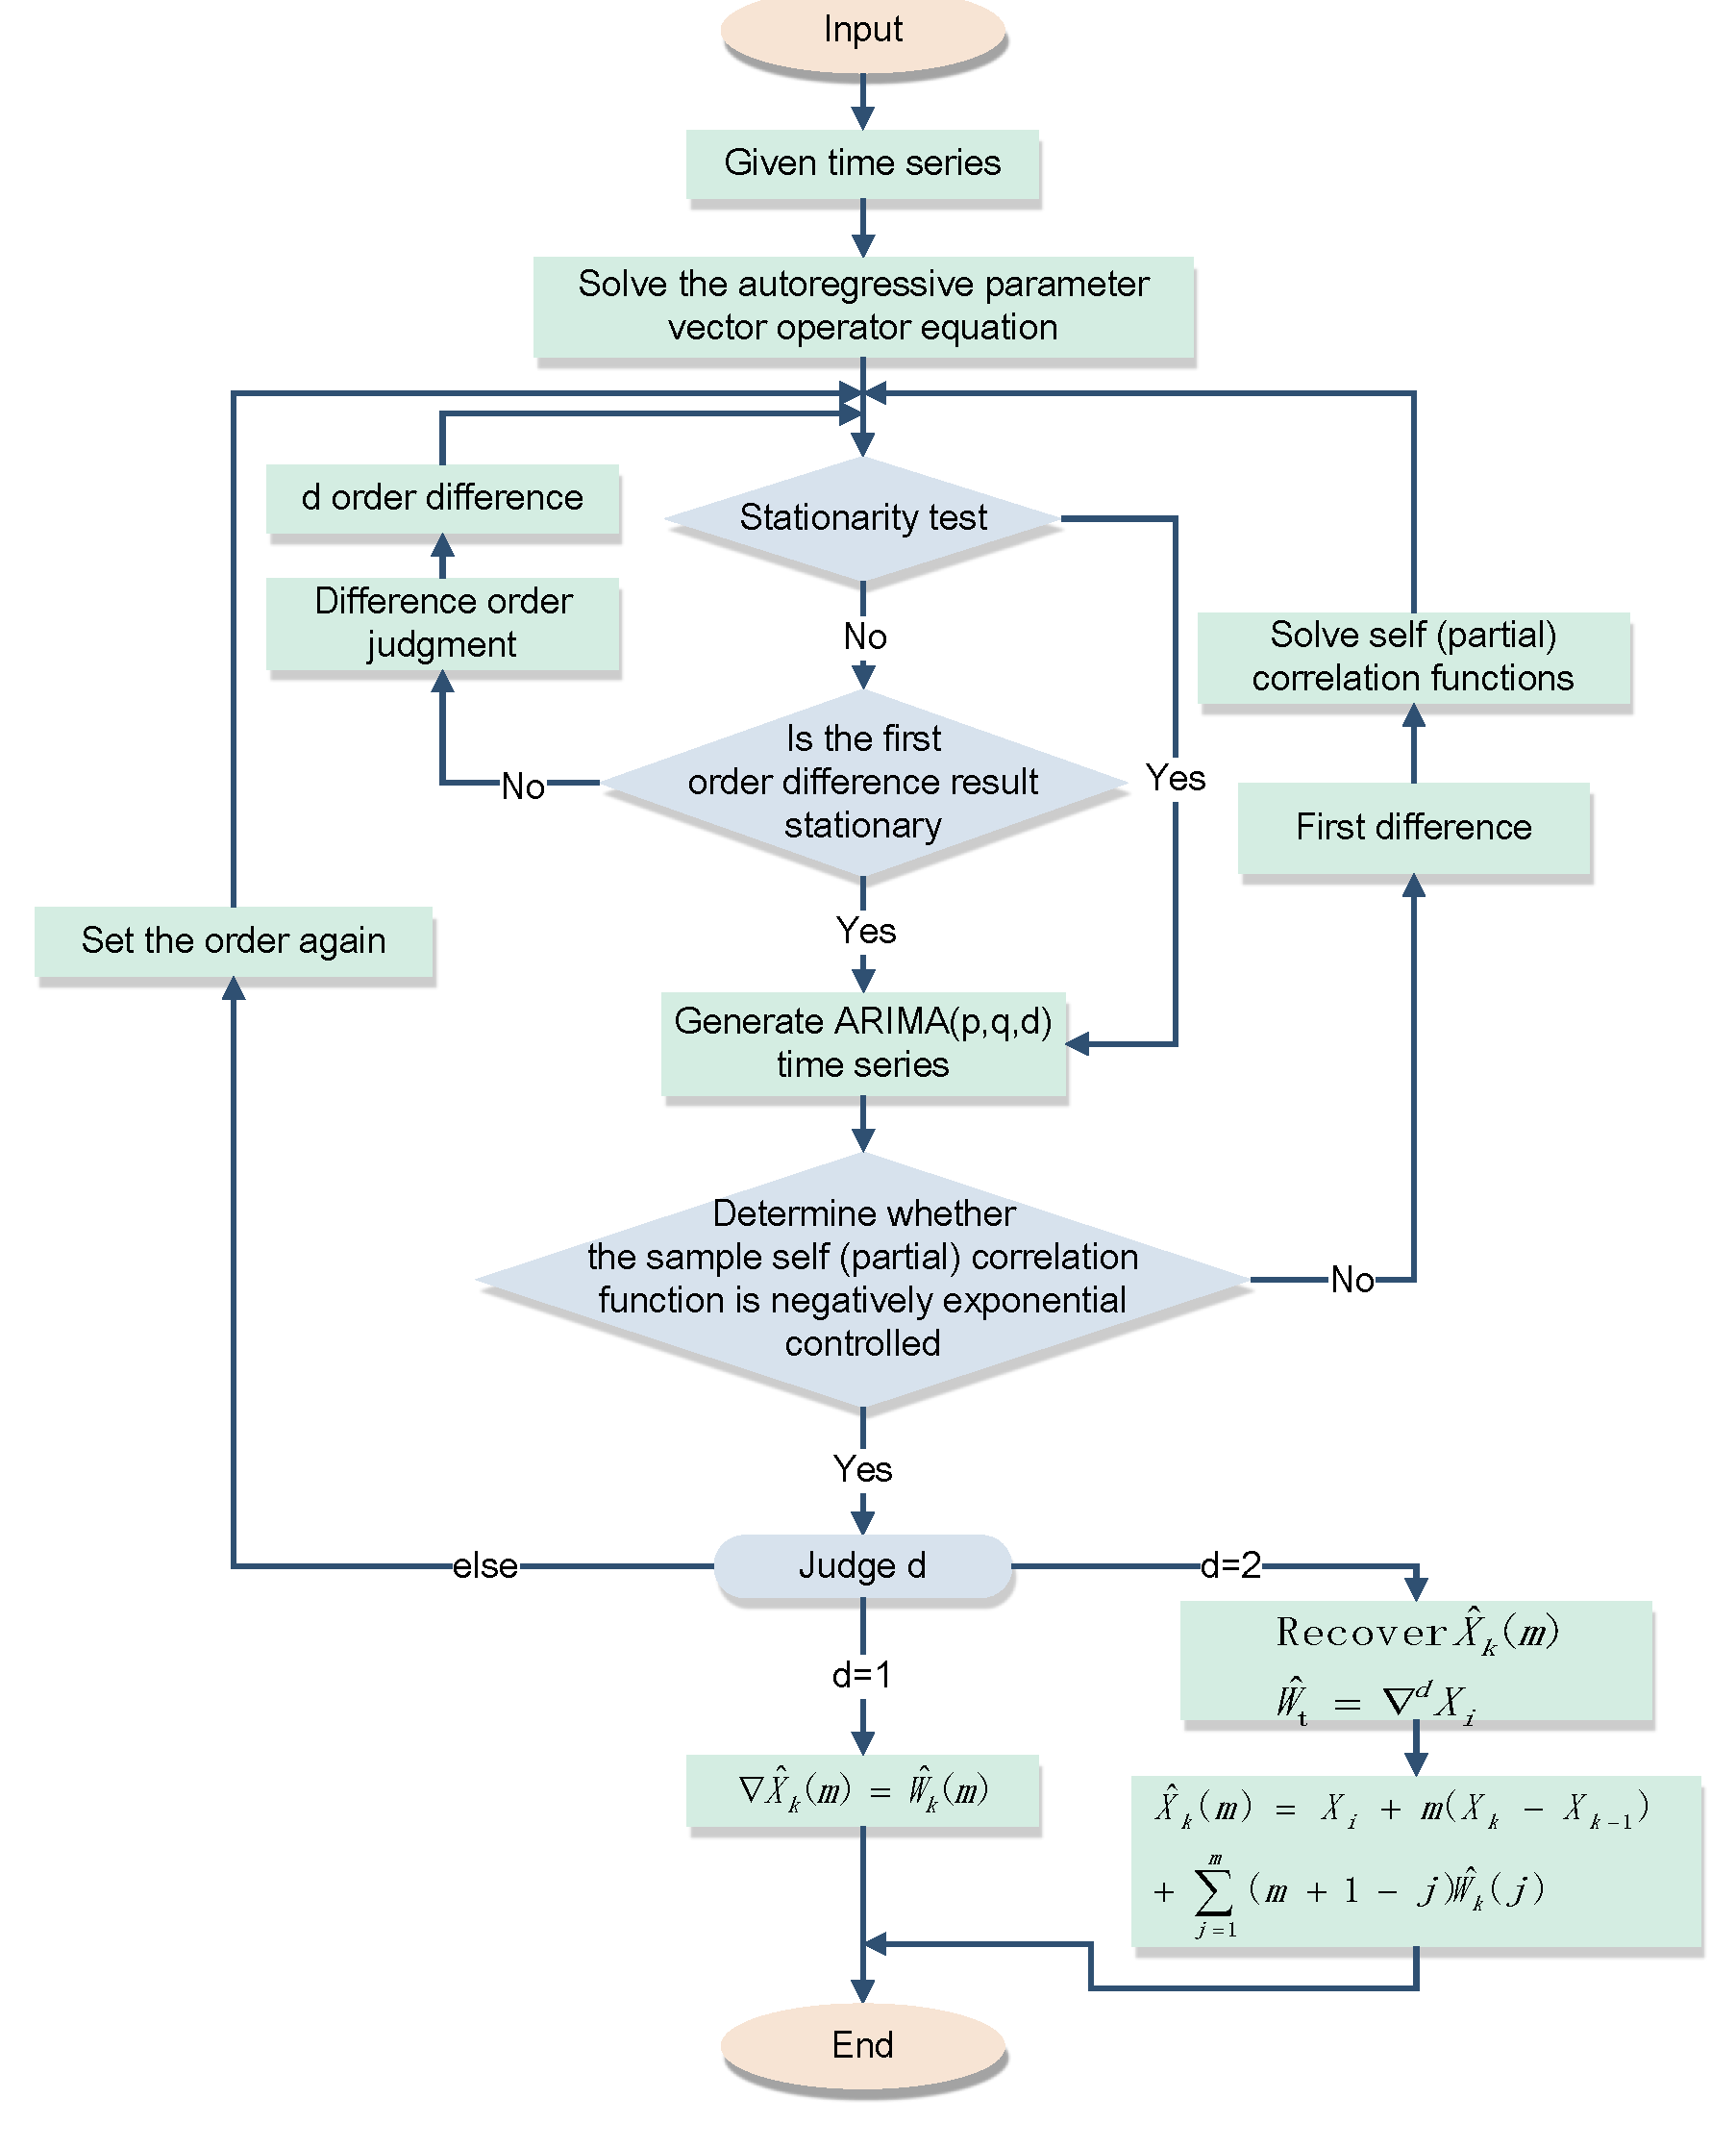
\includegraphics[width =11cm]{codes/ARIMA_裁剪页面.pdf}
    \caption{}
  \end{flushright}
\end{minipage}
\par
$ n $ is the capacity of sample;$ \hat{\sigma_\epsilon^2} $ is the
estimation of $ \sigma_\epsilon^2 $ relating to $ p $ and $ q $.
Suppose $ p = \hat{p}, q = \hat{q} $, such that equation(\ref{AIC}) reaches the minimum,
than we deem the series is $ \mathbf{ARMA}(\hat{p},\hat{q}) $. 
\par
Suppose $ \mathbf{ARMA}(p,q) $ series has an unknown average parameter $ \mu $,
the model becomes
$$
  \phi(B)(X_y-\mu) = \theta(B)\epsilon_t,
$$   
meanwhile, the number of unknown parameters is $ k = p+q+2 $, the AIC is:
choose $ p,q $ such that
\begin{equation}\label{AIC_unknown}
  \min \mathbf{AIC} = n\ln\hat{\sigma_\epsilon^2}+2(p+q+2).
\end{equation}  
In fact, equations(\ref{AIC})and(\ref{AIC_unknown})have the same minimum point $ \hat{p},\hat{q} $.
After that, we usually choose $ p = 1, q = 1 $ to make parameter estimation 
over ARMA model.
\par
It's demonstrated that the differential operation can stabilize 
certain class of non-stationary series. And It's emphasized that 
stationary test must be conducted previously. Stationary test can 
be applied by calculating sample autocorrelation function and 
sample coefficient of partial function. 
\par
If the functions are truncated or trending to 0(meaning being controlled
by negative index), than the series belongs to ARMA model.
\par
If at least one of the functions above is not truncated or trending to 0, than
it's not stationary.
\par
Suppose the series is non-stationary, which can be transformed to 
a stationary series by $ d $ -degree differential operation, denoted
as $ \mathbf{ARIMA}(p,q,d) $ series,than differentiate the sample by
$ d $ -degree:
$$
  W_t = \nabla^dX_t,\quad t = d+1,\dots , n
$$ 
After that, apply stationary test on $ W_t $ and repeat steps above 
until it becomes a stationary series, Than $ W_t $(which is denoted
as $ X_t $ ) complies ARMA model. 
\par
The figures below describe the result of ARIMA model on the 
time series of the size of finless porpoise $ N_t, \quad t = 1\cdots 30 $,
in which the Figure(\ref{ARIMA Sequence}) clearly shows that the number
will decline and settle around 62 in the future 20 years. 

\subsection{Model III: Cellular Automata based population size prediction}

\subsection{Model IV: Gray Forecast model}

\begin{figure}[htbp]
  \centering

  \subfigure[Sample Autocorrelation Function and Sample Partial Autocorrelation Function]{
  \centering
  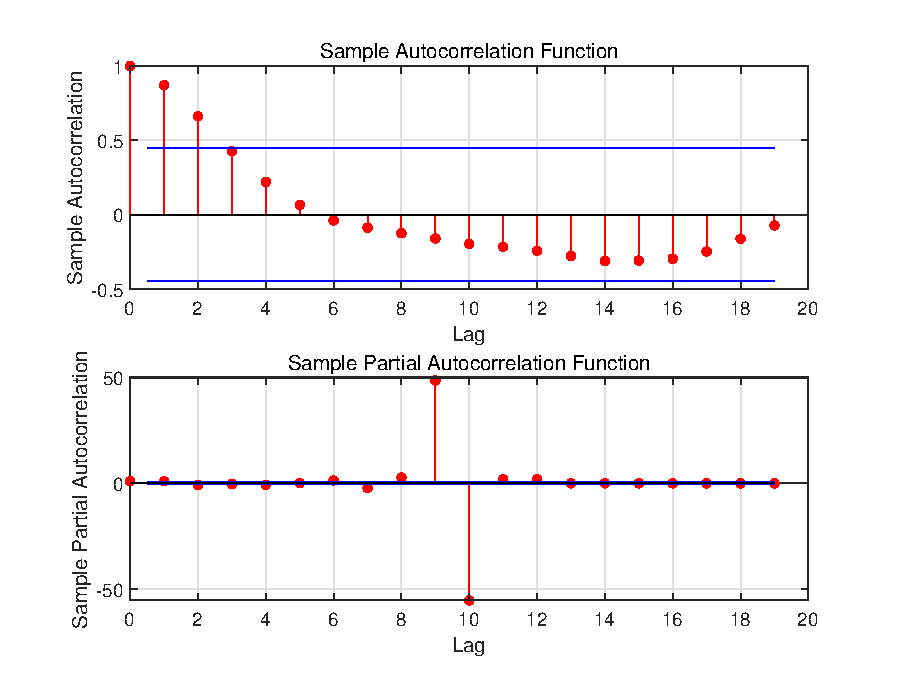
\includegraphics[width = 0.45\textwidth]{codes/1.eps}
  }
\quad
  \subfigure[Sample Autocorrelation Function and Sample Partial Autocorrelation Function]{
  \centering
  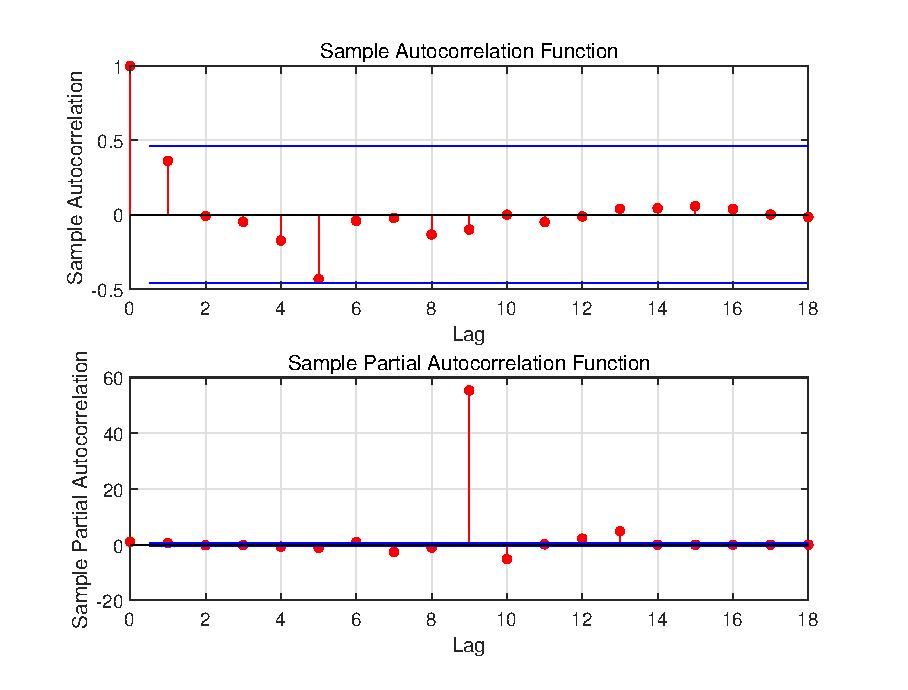
\includegraphics[width = 0.45\textwidth]{codes/3.eps}
  }
\quad
  \subfigure[ARIMA Sequence Prediction of Conservation]{
  \centering
  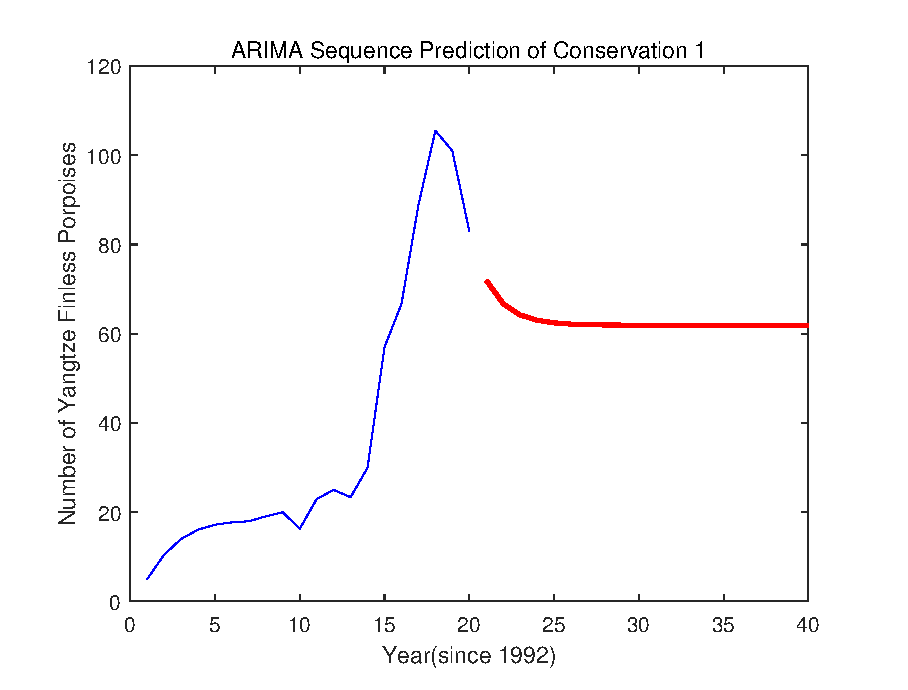
\includegraphics[width = 0.45\textwidth]{codes/2.eps}\label{ARIMA Sequence}
  }
\quad
\subfigure[Standardaized Residuals and QQ figure]{
  \centering
  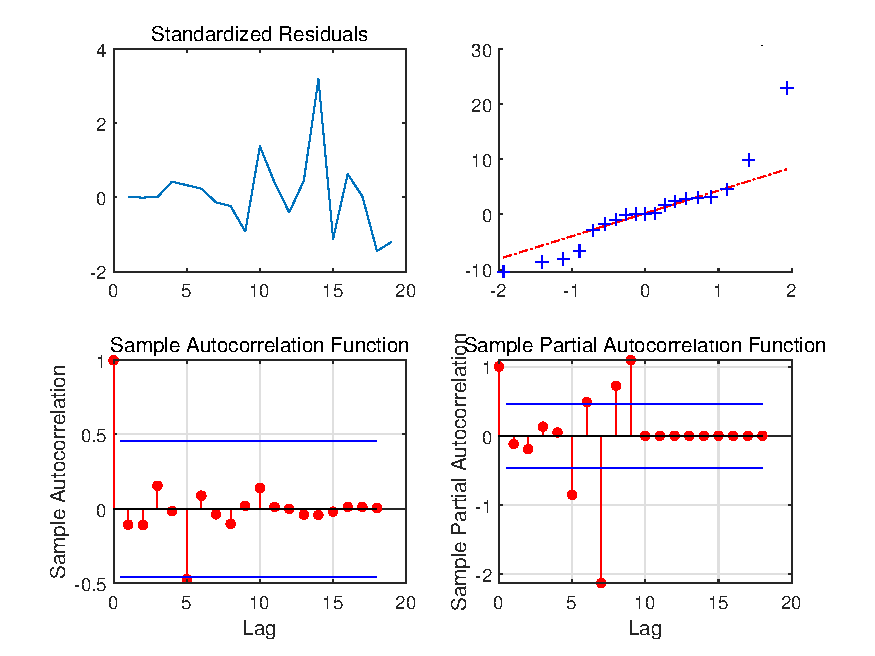
\includegraphics[width =0.45\textwidth]{codes/4.pdf}
}

\end{figure}




\begin{figure}[htbp]
  \centering
  \subfigure[Living Environment Index and Population]{
    \centering
    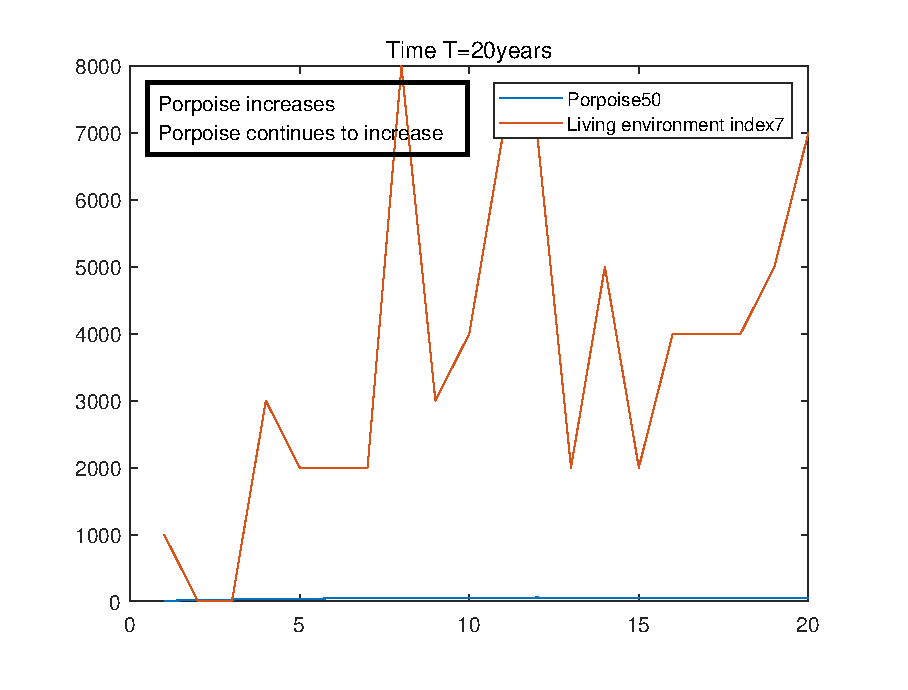
\includegraphics[width = .45\textwidth]{codes/20(1).eps}
    \quad
    }
  \subfigure[Cell Distribution]{
    \centering
    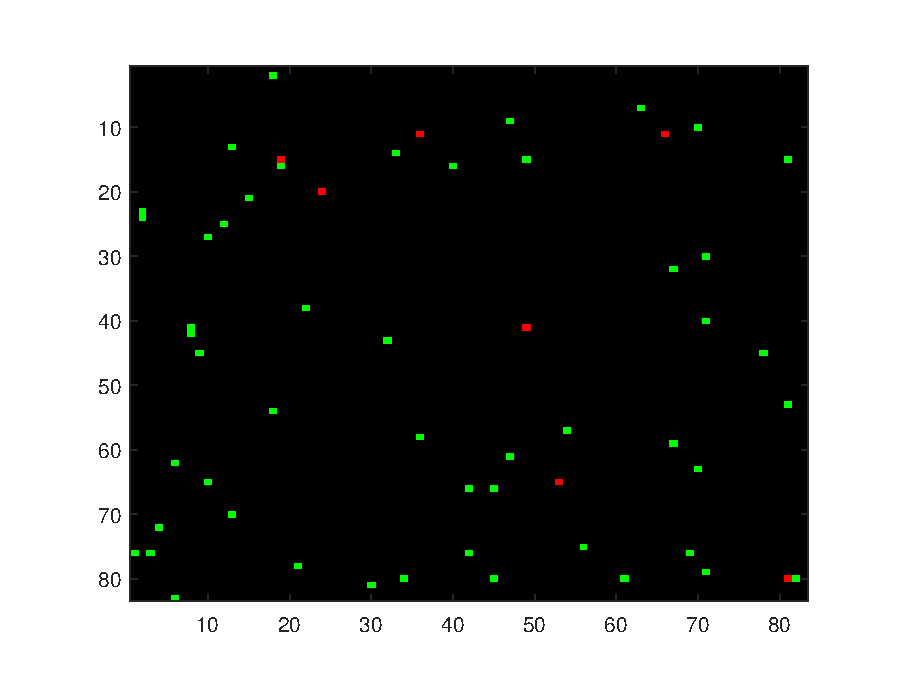
\includegraphics[width=.45\textwidth]{codes/20(2).eps}
  }
\end{figure}





\section{}

















\section{Sensitivity Test}

\section{Evaluation of Model}

\section{Conclusions}

\newpage
\phantomsection\addcontentsline{toc}{section}{Report}\tolerance=500
\memoto{123}
\memofrom{123}
\memodate{\today}

\begin{memo}[report]
  
\end{memo}




\newpage

%这一行是用来将Reference添加到目录的
\phantomsection\addcontentsline{toc}{section}{Refence}\tolerance=500

\bibliographystyle{apacite}
\bibliography{reference.bib}



\newpage


\lhead{\small\sffamily \team}
\rhead{\small\sffamily Page \thepage\ }

\begin{appendices}




\textbf{\textcolor[rgb]{0.98,0.00,0.00}{Input matlab source:}}
\lstinputlisting[language=Matlab]{./codes/lagrange_main.m}
\lstinputlisting[language=Matlab]{./codes/lagrange.m}
\lstinputlisting[language=Matlab]{./codes/ARIMA.m}


\end{appendices}


\end{document}

